\section{Summary of Paper \ref{pap:physics}}
\subsection*{"\nameref{pap:physics}"}
\subsection*{Scope and motivations}
Minimizing the number of regressor variables is often advisable to reduce the risk of overfitting to irrelevant data, aligning with the long-standing principle that ``Nature is simple'' \cite{ljungPerspectivesSystemIdentification2010}. However, this prejudiced approach could also lead to model structures with limited applicability, as certain regression terms may only become significant under specific conditions, such as sailing in wind \cite{abkowitzMEASUREMENTHYDRODYNAMICCHARACTERISTICS1980}.

It was shown in Paper \ref{pap:pit} that it is possible to identify a model from a calm water free running model test through inverse dynamics regression (\autoref{sec:IDR}) together with a cross validation technique to find a truncated model that can predict other types of maneuvers with adequate accuracy. However, it was soon discovered that these models did not generalize well when wind forces were added to the simulations. 

Paper \ref{pap:physics}  investigated this issue using two modular manoeuvring models. One of the models was a data-driven, physics-uninformed (PU) model, akin to the models used in the prior paper (Paper \ref{pap:pit}).
The other model was a physics-informed (PI) model, which incorporated prior knowledge of rudder hydrodynamics to guide the identification toward a more physically correct model. 
The models had identical prediction models for the hull and propeller forces but different models for the rudder forces. The PI model had a deterministic semi-empirical rudder model, while the PU model had a data-driven mathematical rudder model. The ship manoeuvring models were similar to the MMG model \cite{yasukawaIntroductionMMGStandard2015}, apart from the difference in rudder models and some minor enhancements, such as the expression of the surge velocity as a perturbed velocity (see \autoref{sec:prime_system}), allowing for higher-order resistance coefficients.

A brief description of the workflow of Paper \ref{pap:physics} is shown in \autoref{fig:methodology}.
The PI and PU models were identified from free-running model tests using inverse dynamics and regression. A reference model was established to assess physical correctness, where the PI model was instead identified based on VCT data. This reference model, based on CFD, was assumed to be an adequate representation of the ship's physics.
Verification and comparisons between the models were carried out in the free-sailing model tests.
\begin{figure}[h]
  \centering
  %\includesvg[width=\columnwidth, pretex=\scriptsize, height=12cm]{figures/methodology2.svg}
  \includesvg[width=0.9\textwidth, pretex=\centering\fontsize{9.5}{10}]{kappa/images/methodology2.svg}
  \caption{Research workflow, describing how the reference model is identified with regression of VCT data and the PI and PU models are identified with regression of inverse dynamics forces from model tests. Results are then gathered to assess the parameter drift, physical correctness and generalization of the models.}
  \label{fig:methodology}
\end{figure}
The effect of incorporating a deterministic semi-empirical rudder model into the PI model on reducing multicollinearity and improving generalization was examined.
\FloatBarrier
\subsection*{Results and main findings}
Force predictions using reference, PI, and PU models for the states during one of the zigzag10/10 tests with wPCC were compared with the inverse dynamics forces for the same test in \autoref{fig:ID_zigzag10}. The PI and PU models predicted the same total yawing moment $N_D$ and sway force $Y_D$ as the reference model. However, the decomposition of this total yawing moment into components of the hull $N_H$ and the rudder $N_R$ differed significantly between the PU model and the PI and reference models, which were quite similar to each other.

\begin{figure}[h] \centering 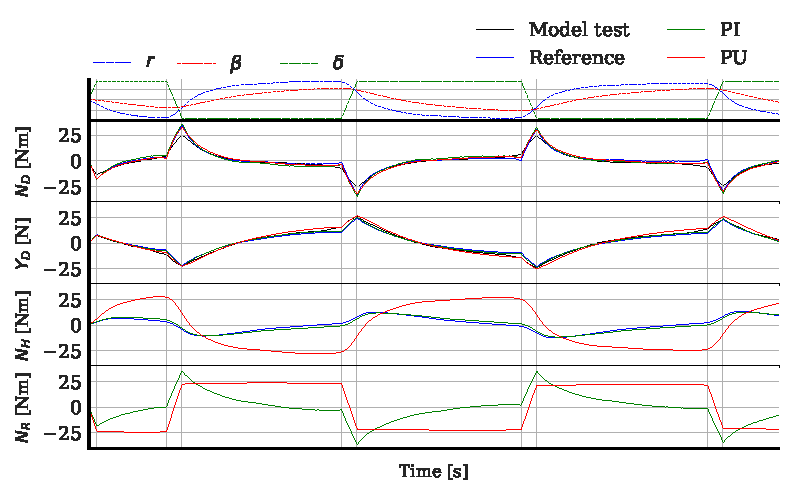
\includegraphics[width=0.9\textwidth]{kappa/images/results.ID_zigzag10.pdf} \caption{ID estimations of $Y_D$ and $N_D$ during a zigzag10/10 model test compared with model predictions.} \label{fig:ID_zigzag10} \end{figure}

The hull forces can be further decomposed into contributions from the drift of the vessel $N_H(v)$ and $Y_H(v)$, and contributions from the yaw rate $N_H(r)$ and $Y_H(r)$, as shown in \autoref{fig:ID_regression_N_decomposition}. It appears that almost all the yawing moments $N_H$ depend on $r$ for the PU model, and almost all the sway force $Y_H$ is generated by $v$. This contrasts with the other two models, where both $v$ and $r$ contribute to $N_H$ and $Y_H$.

\begin{figure}[h] \begin{center} \includesvg[width=0.9\textwidth]{kappa/images/results.hull_force_decomposition_zigzag20.svg} \caption{Decomposition of hull forces and moments during a zigzag20/20 test for parameters related to drift, yaw rate, and the prediction models.} \label{fig:ID_regression_N_decomposition} \end{center} \end{figure}

Thus, the PU model not only misrepresents the decomposition between rudder and hull forces but also incorrectly separates the contributions of drift and yaw rate within the hull force model. However, this is not a significant problem during the zigzag tests, where the drift and yaw rate are highly correlated, as seen from the phase plot in \autoref{fig:phase_portrait}. This correlation can also explain why the completely data-driven model from the previous paper (Paper \ref{pap:pit}) performed well despite the erroneous decomposition.

\begin{figure}[h] \centering \includesvg{figures/multicollineraity.multicollinearity.svg} \caption{Phase portrait showing the combination of drift angle and yaw rate for zigzag10/10 and zigzag20/20 wPCC model tests.} \label{fig:phase_portrait} \end{figure}

However, when the ship is exposed to wind, causing changes in drift, the erroneous decomposition of the PU model becomes apparent, as shown in \autoref{fig:result_wind_state}. The PI model exhibits better alignment with the reference model under wind conditions. Introducing a semi-empirical rudder model seems to have guided the identification toward a more physically accurate model, with lower multicollinearity and better generalization from calm water zigzag tests to wind conditions.

\begin{figure}[h!] 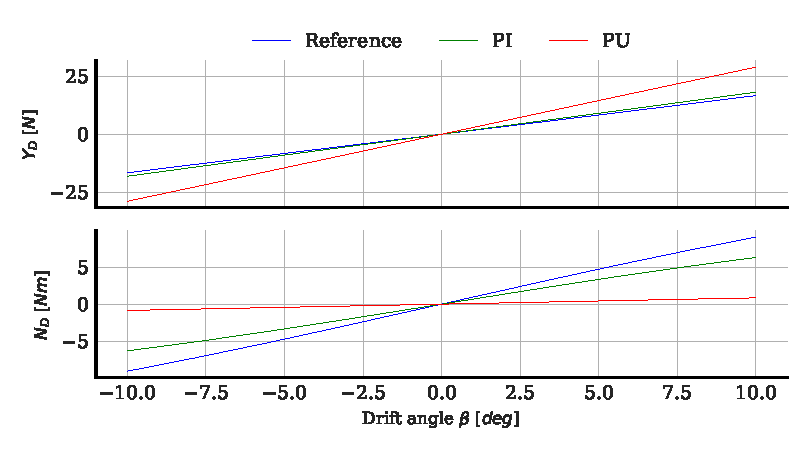
\includegraphics[width=\textwidth]{kappa/images/result_wind_state.forces.pdf} \caption{Total sway force and yawing moment from the wPCC models at various drift angles.} \label{fig:result_wind_state} \end{figure}

\FloatBarrier \clearpage